\documentclass{article}

\usepackage[utf8]{inputenc}
\usepackage{longtable}
\usepackage{authblk}
\usepackage{adjustbox}
\usepackage{natbib}

\title{LOS INDICES DE COLOMBIA}
% autores
\renewcommand\Authand{, y }
\author[1]{\normalsize Laura Valeria Vanegas García}

\affil[1]{\small  Facultad de Ingeniería,Universidad de los Andes\\
\texttt{{lv.vanegas10}@uniandes.edu.co}}

\date{29 de Junio de 2018}

\usepackage{Sweave}
\begin{document}
\Sconcordance{concordance:paper_version1.tex:paper_version1.Rnw:%
1 18 1 1 0 18 1 1 8 7 1 1 5 14 0 1 2 6 1 1 15 1 2 9 1 1 14 1 2 8 1 1 5 %
12 0 1 2 4 1 1 8 13 0 1 2 5 1 2 2 12 1 1 5 1 1 1 4 31 0 1 2 10 1 1 21 1 %
1 1 18 5 1 1 14 1 2 9 1}


\maketitle

\begin{abstract}
Este es mi proyecto final para el curso de verano IIN4347 de la Universidad ded los Andes para 2018-19. Este es mi primer trabajo en exploracion y modelamiento de indices usando LATEX. Este trabajo lo he hecho bajo la filosofía de trabajo replicable. Este es mi proyecto final para el curso de verano IIN4347 de la Universidad ded los Andes para 2018-19. Este es mi primer trabajo en exploracion y modelamiento de indices usando LATEX. Este trabajo lo he hecho bajo la filosofía de trabajo replicable.
\end{abstract}

\section*{Introducción}

En este documento presento mi investigacion sobre diversos indices sociales en Colombia. Los indices fueron extraidos de wikipedia y se realizó preprocesamiento en Python con ayuda de la librería Pandas. En este documento presento mi investigacion sobre diversos indices sociales en Colombia. Los indices fueron extraidos de wikipedia y se realizó preprocesamiento en Python con ayuda de la librería Pandas. 

En este documento presento mi investigacion sobre diversos indices sociales en Colombia. Los indices fueron extraidos de wikipedia y se realizó preprocesamiento en Python con ayuda de la librería Pandas.En este documento presento mi investigacion sobre diversos indices sociales en Colombia. Los indices fueron extraidos de wikipedia y se realizó preprocesamiento en Python con ayuda de la librería Pandas. En este documento presento mi investigacion sobre diversos indices sociales en Colombia. Los indices fueron extraidos de wikipedia y se realizó preprocesamiento en Python con ayuda de la librería Pandas.

Comencemos viendo que hay en la sección \ref{univariada} en la página \pageref{univariada}.

\clearpage


\section{Exploración Univariada}\label{univariada}

Esta es la sección de exploración univariada. En esta sección exploro cada índice.Esta es la sección de exploración univariada. En esta sección exploro cada índice. Esta es la sección de exploración univariada. En esta sección exploro cada índice. 

Además de la distribución de los variable, es importante saber el valor central. Como los valores son de naturaleza ordinal debemos pedir la {\bf mediana} y otras medidas de posición (como los \emph{cuartiles}, los que no pediremos pues son pocos valores). La mediana de cada variable la mostramos en la Tabla \ref{stats} en la página \pageref{stats}.


% Table created by stargazer v.5.2.2 by Marek Hlavac, Harvard University. E-mail: hlavac at fas.harvard.edu
% Date and time: vi., jun. 29, 2018 - 18:54:32
\begin{table}[!htbp] \centering 
  \caption{Medidas estadísticas} 
  \label{stats} 
\begin{tabular}{@{\extracolsep{5pt}}lcccc} 
\\[-1.8ex]\hline 
\hline \\[-1.8ex] 
Statistic & \multicolumn{1}{c}{N} & \multicolumn{1}{c}{Median} & \multicolumn{1}{c}{Min} & \multicolumn{1}{c}{Max} \\ 
\hline \\[-1.8ex] 
IDH & 32 & 0.804 & 0.691 & 0.879 \\ 
Población.Cabecera & 32 & 717,197 & 13,090 & 10,070,801 \\ 
Población.Resto & 32 & 268,111.5 & 21,926 & 1,428,858 \\ 
\hline \\[-1.8ex] 
\end{tabular} 
\end{table} 
A continuación, se muestra el histograma en la Figura \ref{histplots} en la página \pageref{histplots}.de las variables IDH, Población cabecera y Población Restante:

%%%%% figure
\begin{figure}[h]
\centering
\begin{adjustbox}{width=7cm,height=7cm,clip,trim=1.5cm 0.5cm 0cm 1.5cm}
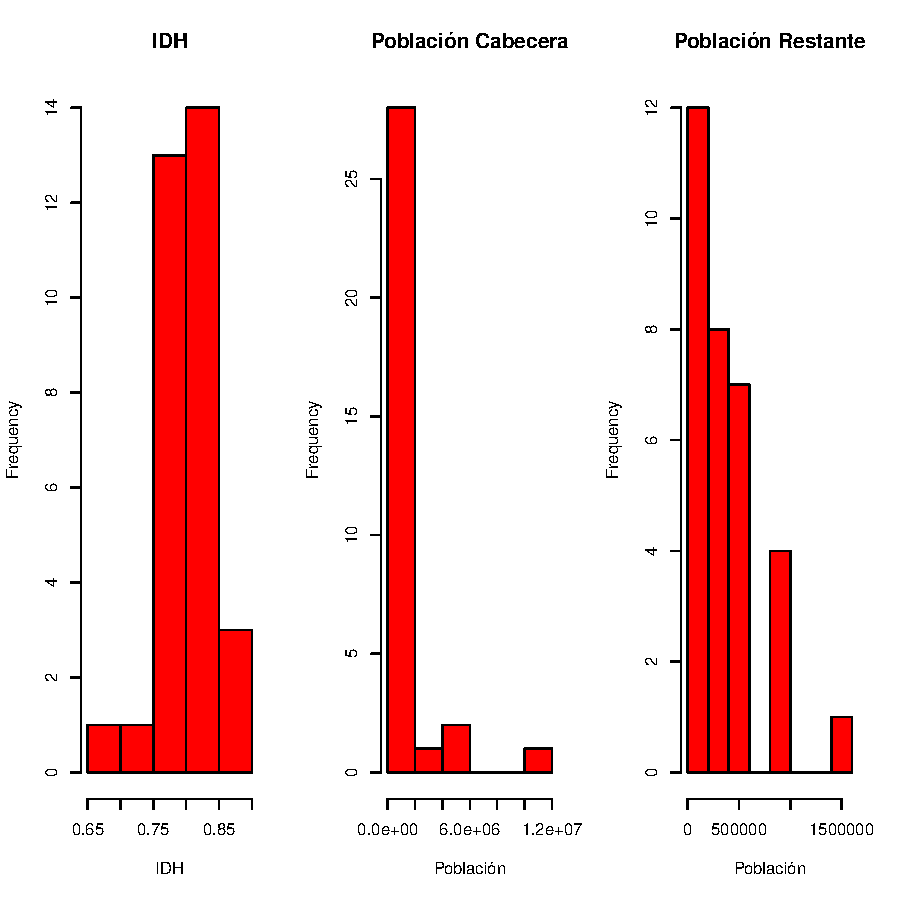
\includegraphics{paper_version1-histograms}
\end{adjustbox}
\caption{Histogramas}
\label{histplots}
\end{figure}

Dado el sesgo de las pobaciones, podriamos transformarla para que se acerque a la normalidad. En la Figura \ref{histplotsNorm} en la página \pageref{histplotsNorm}, se muestran los histogramas con las poblaciones normalizadas con una transformación de logarítmo. 

\begin{figure}[h]
\centering
\begin{adjustbox}{width=7cm,height=7cm,clip,trim=1.5cm 0.5cm 0cm 1.5cm}
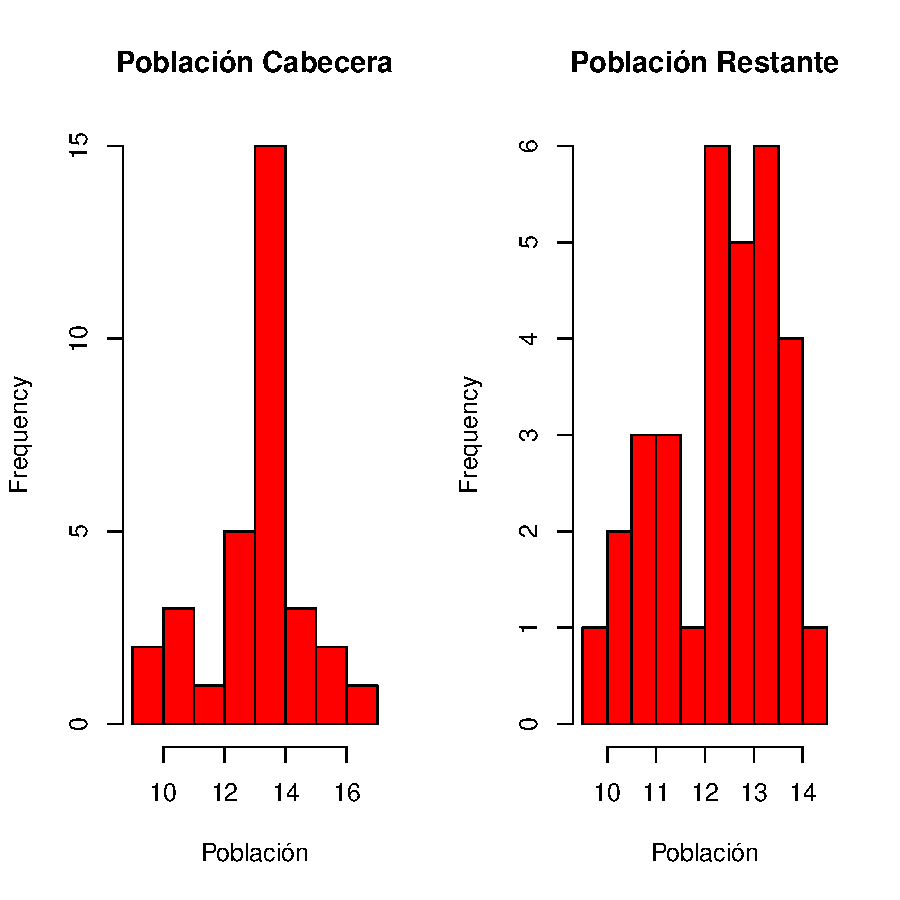
\includegraphics{paper_version1-histogramsNorm}
\end{adjustbox}
\caption{Histogramas Población Normalizados }
\label{histplotsNorm}
\end{figure}

\section{Exploración Bivariada}\label{bivariada}

En este trabajo estamos interesados en el impacto de los otros indices en el nivel de Democracia. Veamos las relaciones bivariadas que tiene esta variable con todas las demás:

% Table created by stargazer v.5.2.2 by Marek Hlavac, Harvard University. E-mail: hlavac at fas.harvard.edu
% Date and time: vi., jun. 29, 2018 - 18:54:37
\begin{table}[!htbp] \centering 
  \caption{Correlación de Democracia con las demás variables} 
  \label{corrDem} 
\begin{tabular}{@{\extracolsep{5pt}} cc} 
\\[-1.8ex]\hline 
\hline \\[-1.8ex] 
cabeLog & restoLog \\ 
\hline \\[-1.8ex] 
$0.487$ & $0.177$ \\ 
\hline \\[-1.8ex] 
\end{tabular} 
\end{table} 

Veamos la correlación entre las variables independientes:


% Table created by stargazer v.5.2.2 by Marek Hlavac, Harvard University. E-mail: hlavac at fas.harvard.edu
% Date and time: vi., jun. 29, 2018 - 18:54:37
\begin{table}[!htbp] \centering 
  \caption{Correlación entre variables independientes} 
  \label{corrTableX} 
\begin{tabular}{@{\extracolsep{5pt}} ccc} 
\\[-1.8ex]\hline 
\hline \\[-1.8ex] 
 & cabeLog & restoLog \\ 
\hline \\[-1.8ex] 
cabeLog & 1 &  \\ 
restoLog & 0.8 & 1 \\ 
\hline \\[-1.8ex] 
\end{tabular} 
\end{table} 
Lo visto en la Tabla \ref{corrTableX} se refuerza claramente en la Figura \ref{corrPlotX}.

\begin{figure}[h]
\centering
\begin{adjustbox}{}
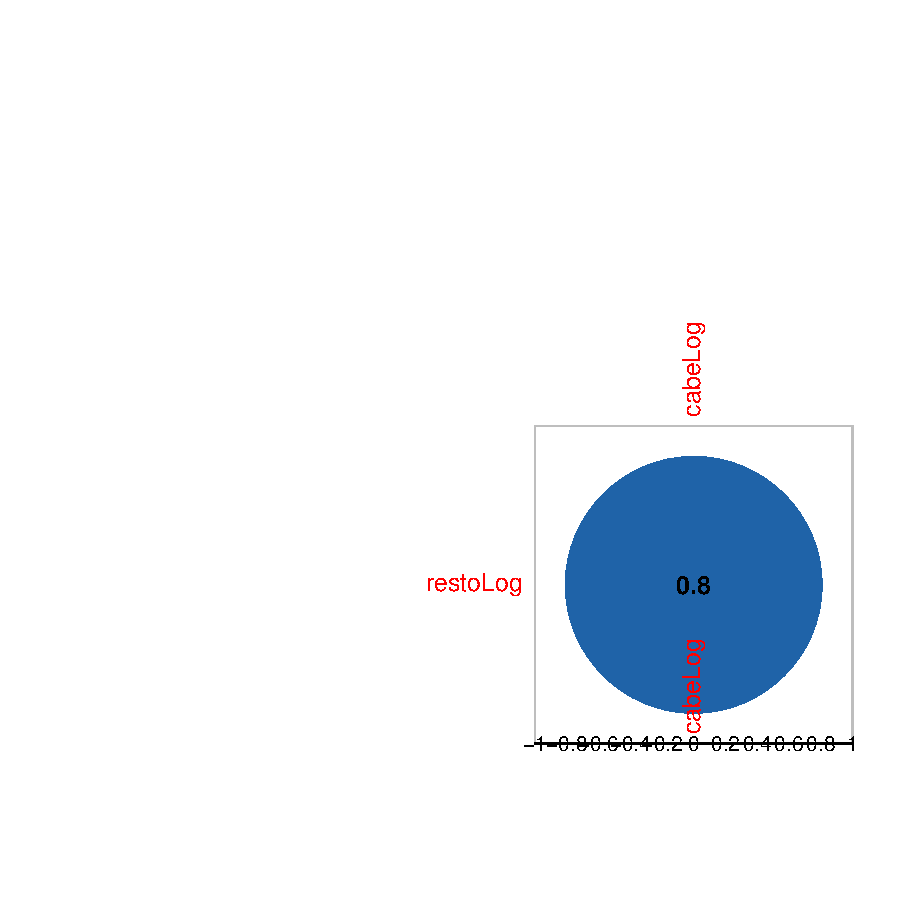
\includegraphics{paper_version1-corrPlotX}
\end{adjustbox}
\caption{Correlación entre predictores}
\label{corrPlotX}
\end{figure}

\section{Modelos de Regresión}

Finalmente, vemos los modelos propuestos. Primero sin poblacion resto, luego con esta. Los resultados se muestran en la Tabla \ref{regresiones} de la página \pageref{regresiones}. Finalmente, vemos los modelos propuestos. Primero sin poblacion resto, luego con esta. Los resultados se muestran en la Tabla \ref{regresiones} de la página \pageref{regresiones}.Finalmente, vemos los modelos propuestos. 

Primero sin poblacion resto, luego con esta. Los resultados se muestran en la Tabla \ref{regresiones} de la página \pageref{regresiones}.Finalmente, vemos los modelos propuestos. Primero sin poblacion resto, luego con esta. Los resultados se muestran en la Tabla \ref{regresiones} de la página \pageref{regresiones}.

Finalmente, vemos los modelos propuestos. Primero sin poblacion resto, luego con esta. Los resultados se muestran en la Tabla \ref{regresiones} de la página \pageref{regresiones}.Finalmente, vemos los modelos propuestos. Primero sin poblacion resto, luego con esta. Los resultados se muestran en la Tabla \ref{regresiones} de la página \pageref{regresiones}.



% Table created by stargazer v.5.2.2 by Marek Hlavac, Harvard University. E-mail: hlavac at fas.harvard.edu
% Date and time: vi., jun. 29, 2018 - 18:54:37
\begin{table}[!htbp] \centering 
  \caption{Modelos de Regresión} 
  \label{regresiones} 
\begin{tabular}{@{\extracolsep{5pt}}lcc} 
\\[-1.8ex]\hline 
\hline \\[-1.8ex] 
 & \multicolumn{2}{c}{\textit{Dependent variable:}} \\ 
\cline{2-3} 
\\[-1.8ex] & \multicolumn{2}{c}{IDH} \\ 
\\[-1.8ex] & (1) & (2)\\ 
\hline \\[-1.8ex] 
 cabeLog & 0.013$^{***}$ & 0.031$^{***}$ \\ 
  & (0.004) & (0.007) \\ 
  & & \\ 
 restoLog &  & $-$0.030$^{***}$ \\ 
  &  & (0.010) \\ 
  & & \\ 
 Constant & 0.634$^{***}$ & 0.766$^{***}$ \\ 
  & (0.055) & (0.065) \\ 
  & & \\ 
\hline \\[-1.8ex] 
Observations & 32 & 32 \\ 
R$^{2}$ & 0.238 & 0.425 \\ 
Adjusted R$^{2}$ & 0.212 & 0.385 \\ 
Residual Std. Error & 0.037 (df = 30) & 0.033 (df = 29) \\ 
F Statistic & 9.347$^{***}$ (df = 1; 30) & 10.706$^{***}$ (df = 2; 29) \\ 
\hline 
\hline \\[-1.8ex] 
\textit{Note:}  & \multicolumn{2}{r}{$^{*}$p$<$0.1; $^{**}$p$<$0.05; $^{***}$p$<$0.01} \\ 
\end{tabular} 
\end{table} 
Podemos sacar conclusiones al observar los resultados de las  regresiones en \ref{regresiones}

\section{Exploración Espacial}

Calculemos conglomerados de regiones, usando toda la información de las tres variables.Usaremos la tecnica de k-means propuesta por \cite{macqueen_methods_nodate}. Calculemos conglomerados de regiones, usando toda la información de las tres variables.Usaremos la tecnica de k-means propuesta por \cite{macqueen_methods_nodate}. Calculemos conglomerados de regiones, usando toda la información de las tres variables.Usaremos la tecnica de k-means propuesta por \cite{macqueen_methods_nodate}.Calculemos conglomerados de regiones, usando toda la información de las tres variables.Usaremos la tecnica de k-means propuesta por \cite{macqueen_methods_nodate}. Calculemos conglomerados de regiones, usando toda la información de las tres variables.Usaremos la tecnica de k-means propuesta por \cite{macqueen_methods_nodate}.

Calculemos conglomerados de regiones, usando toda la información de las tres variables.Usaremos la tecnica de k-means propuesta por \cite{macqueen_methods_nodate}. Calculemos conglomerados de regiones, usando toda la información de las tres variables.Usaremos la tecnica de k-means propuesta por \cite{macqueen_methods_nodate}. Calculemos conglomerados de regiones, usando toda la información de las tres variables.Usaremos la tecnica de k-means propuesta por \cite{macqueen_methods_nodate}.Calculemos conglomerados de regiones, usando toda la información de las tres variables.Usaremos la tecnica de k-means propuesta por \cite{macqueen_methods_nodate}. Calculemos conglomerados de regiones, usando toda la información de las tres variables.Usaremos la tecnica de k-means propuesta por \cite{macqueen_methods_nodate}.

A continuación se muestra el mapa de Colombia con ubicaciones.






\begin{figure}[h]
\centering
\begin{adjustbox}{width=12cm,height=12cm,clip,trim=0cm 0cm 0cm 0cm}
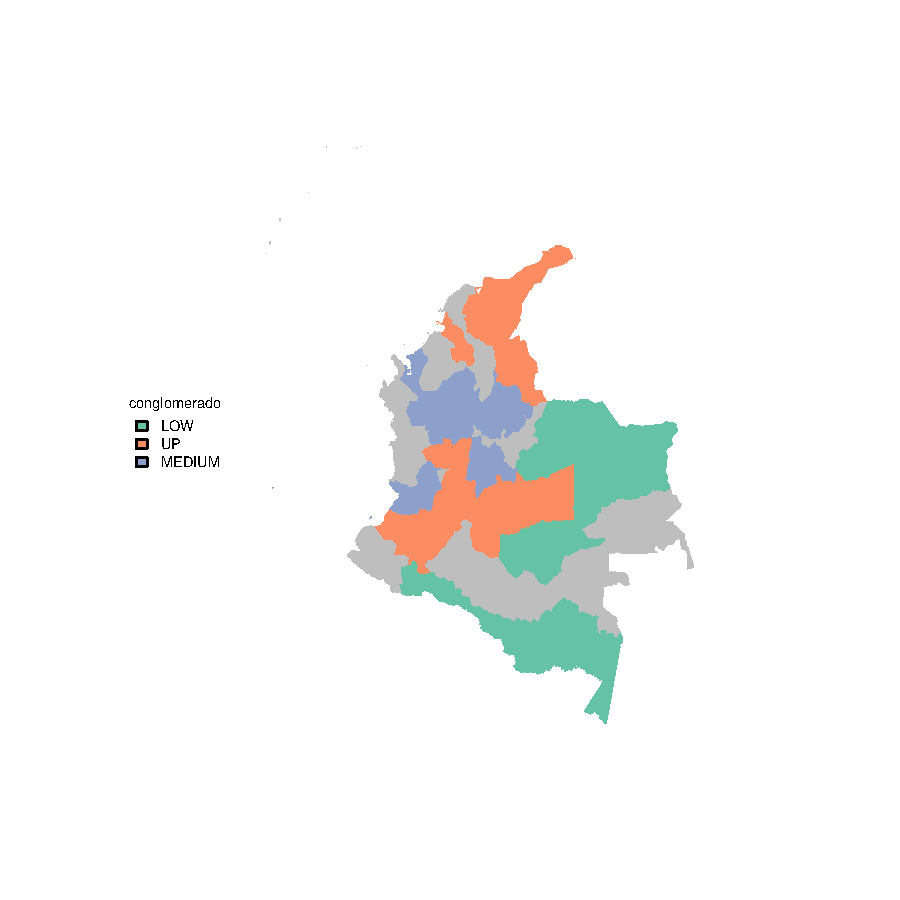
\includegraphics{paper_version1-plotMap1}
\end{adjustbox}
\caption{Departamentos conglomerados segun sus indicadores}\label{clustmap}
\end{figure}


\bibliographystyle{abbrv}
%\renewcommand{\refname}{Bibliography}
\bibliography{Colombia}

\end{document}
